% !TEX root = paper.tex
% !TEX encoding = UTF-8 Unicode
% -*- coding: UTF-8; -*-
% vim: set fenc=utf-8
% !TEX spellcheck = en-US
\section{Methods}

A current hypothesis regarding active vision is that visual scenes most often consist of a single visual object of interest. Take for instance the case of a conversation with a friend at a noisy cafe. To ease the understanding of his voice and emotion you will track his face despite all the remaining sensory clutter by scanning relevant parts of his face with your gaze. Such a visual experience can be simplified in a manner reminiscent to psychophysical experiments: An observer is asked to classify digits (for instance as taken from the MNIST database) as they are shown on a computer display. However, these digits can be placed at a random positions on the display, and visual clutter is added as a background to the image (see Figure~\ref{fig:intro}-A) opening the possibility that the position of this object could be detected in the clutter without being able to identify it before making a saccade to it. This defines more precisely our problem: how do we identify a small object in a large image while not knowing \emph{a priori} its position?

\if 0\CNS
This joint problem of localization and identification is the classical problem of visual search in neuroscience. Such problem is very general and can address complex questions such as "find the green bottle on the table". Here, we will restrict ourselves to a simple "feature search"~\citep{Treisman80}. Such a problem found many solutions in computer vision. Notably, recent advances in deep-learning have provided with efficient models such as faster-RCNN~\citep{Ren17} or YOLO~\citep{Redmon15}. This last implementation is particularly interesting as it predicts in the image the probability of proposed bounding boxes around the visual object. While rapid, the amount of such boxes greatly increases with image size and necessitates a dedicated hardware. When limiting our problem to a few objects of interest in the image, this strategy amounts to a classical problem in neuroscience, that is, the transformation of a luminous image into a saliency map~\citep{Itti01}. Such a computation is essential to understand and predict saccades but also as models of attention. Recently, deep learning methods have extended this type of model by learning to extimate saliency maps over large databases of natural images~\citep{Kummerer16}. While these methods are efficient at predicting the probability of fixation, they miss an essential point in the action perception loop: They operate on the full image while the retina operates on the non-uniform, foveated sampling of visual space (see Figure~\ref{fig:intro}-B). Herein, we believe that this fact is an essential factor to reproduce and understand this active vision process.

An interesting perspective is given with previous modeling of such foveated sensors. The non-uniform sampling of visual space is usually modeled as a log-polar conformal mapping~\citep{Traver10} which has a long history in computer vision and robotics. A first property of this mapping is the separation between the foveal and the peripheral areas as we defined above. This transformation has also other notable properties, such as the correspondence by way of translations in the radial and angular directions to respectively rotations and scalings in the visual domain. However, this sensor is most often not coupled to an action (but see~\citep{ref needed)}. In this paper, we aim at addressing the fragmentation of these different approaches respective to their fields (Machine learning, neuroscience, robotics) to propose an integrated computational model of foveated active vision.
\fi
%------------------------------%
%: see Figure~\ref{fig:intro}
\begin{figure}%[!ht]%%[p!]
	%\centering{
	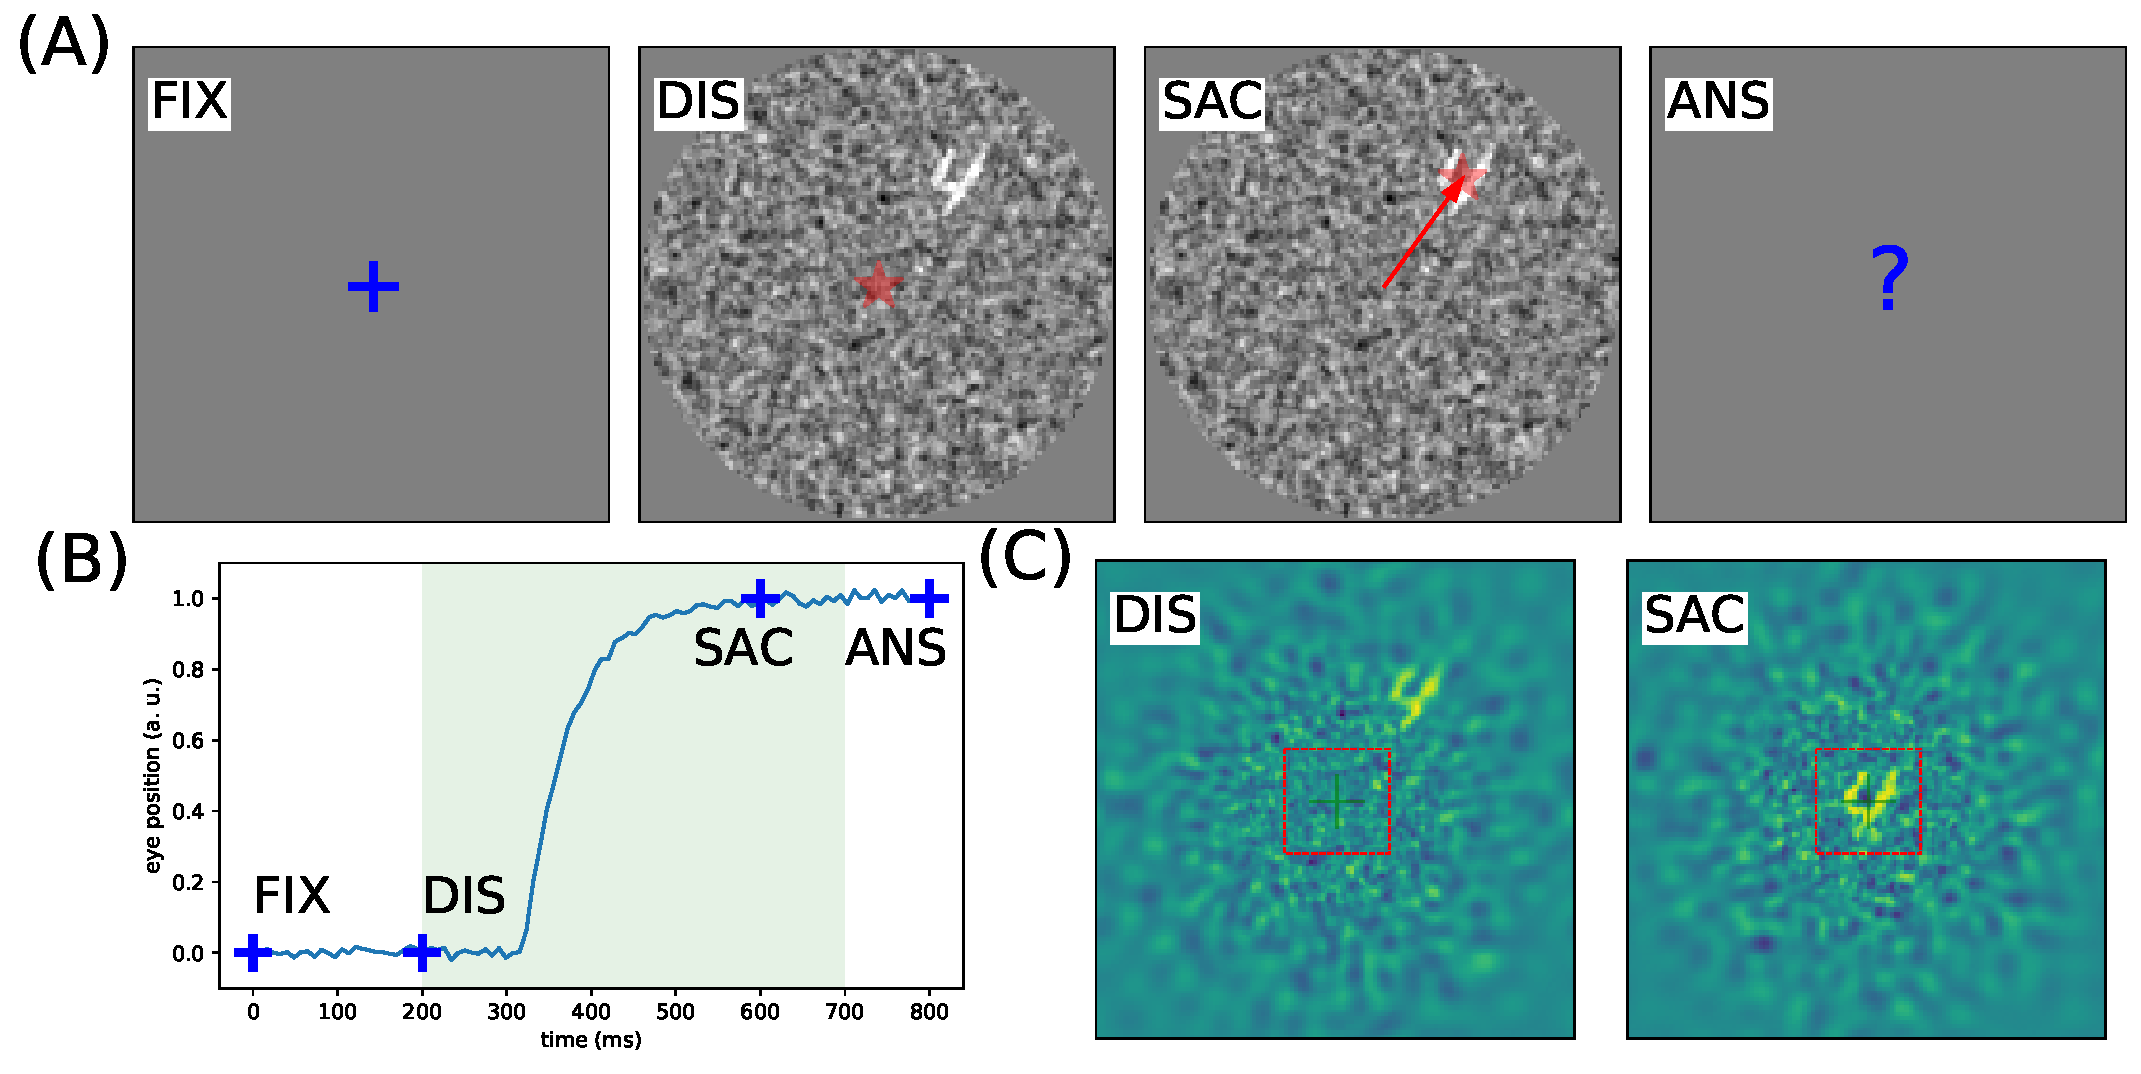
\includegraphics[width=\linewidth]{fig_intro}
	%}
	\caption{
		{\bf Problem setting}: In ecological settings, the visual system faces a tricky problem when searching for \emph{any} target in a cluttered environment. It is synthesized in the following experiment:
		(A)~After a fixation period ('FIX') of $200\ms$, an observer is presented with a luminous display ('DIS') showing a single target from a known class (here digits) and at a random position. The display is presented for a short period, that is enough to perform one saccade on the potential target ('SAC'). \if 0\CNS In particular, the configuration of the display is such that by adding clutter and reducing the size of the digit it may become necessary to perform a saccade to be able to identify the digit. Finally, the observer identifies the digit ('ANS'). \fi %
		(B)~Prototypical trace of a saccadic eye movement to the target position.\if 0\CNS In particular, we show the fixation window used to ensure fixation during that window (green shaded area). \fi (C)~Simulated reconstruction of the visual information from the retinotopic map at respectively ('DIS') the onset of the display and ('SAC') after a (successful) saccade. \if 0\CNS This demonstrates that the position of the target has to be inferred from a degraded (sampled) image ('DIS') and that a correct identification is mediated by the action to the location of the target \emph{before seeing it}, that is before being able to actually be able to identify the target.\fi
		\label{fig:intro}}%
\end{figure}%
%%------------------------------%



\if 0\CNS

The visual scene is here made of a foreground (the target) and a noisy background. An agent controls a focal visual sensor that can move over the visual scene through saccades. 
% both the visual features and the expected target position to be expressed in log-polar coordinates. 
On the primary visual side, local visual features (first and second order orientation filters) are radially organized around the center of fixation, with small and tightened receptive fields at the center and more large and scarce receptive fields at the periphery. The issued observation vector $\boldsymbol{x}$ compresses the original image by about 90\%, with high spatial frequencies preserved at the center and only low spatial frequencies conserved at the periphery. 
%The target accuracy map is also organized radially in a log-polar fashion, making the target position estimate more precise at the center and fuzzier at the periphery. This modeling choice is reminiscent of the approximate log-polar organization of the superior colliculus (SC) motor map {\bf[TODO:REF]}. 
%This retinotopic organization is preserved along the visuo-motor pathway as expected from observations {\bf[TODO:REF]}.
\fi

\if 1\CNS
In an active inference setup, it is assumed that, before taking a decision, the consequence of every saccade should be analyzed by the agent through model inversion,  with each saccade expectedly providing a new visual sample from a given scene statistics, that may increase the understanding of the scene (here the target position and category). Though the effect of action is too complex to be inferred from a generative model, we assume here that it is trained by sampling, i.e. by "trial and error". 
As such, we start as in~\citep{Friston12} by a probabilistic formulation, and use the fundamental hypothesis outlined in Figure~\ref{fig:intro}: the position of an object is independent from its identity. This property is strictly true in our setting and is very generic in vision for simple classes (such as digits) and simple displays\if 0\CNS (but see~\citep{Vo12} for more complex visual scene grammars)\fi . From this independence hypothesis, we may separate the two inter-related tasks (identification vs localization) in two separate pathways with different morphologies (respectively foveal and peripheral). Note that from the retinotopic projection of the visual information, this independence is conditional on action: These pathways should update their beliefs upon decisions made in each respective pathway.
%A first simplifying assumption is a separation of the position and category inferences in two separate pathways, namely the ``What'' and the ``Where'' pathways. 
The agent visual categorical pathway (the ``What'' pathway) is supposed to be realized by a classifier, that mostly processes the central pixels to identify the target category. This central classifier, that is not implemented in our setup, should display a high accuracy at the center, and a shortly decreasing accuracy with target eccentricity, as shown in figure \ref{fig:results}{\bf D}.
In contrast, the visual orientation pathway (the ``Where'' pathway) takes the full visual field into account in order to tell whether a target is present at the different peripheral locations, in order to monitor future saccades. 
A second simplifying assumption is that the putative effect of a saccade should be condensed in a figure, namely the \emph{accuracy}, that is a statistics over the (scene understanding) benefit obtained from past saccades in the same context. In detail, the primary visual information should be transformed so as to predict how accurate the categorical classifier will be after the saccade is carried out. The set of all possible saccade predictions should form an \emph{accuracy map}.
An accuracy map abstracts here a full sequence of operations, including (i) an initial visual examination, followed by (ii) a decision, (iii) a saccade realization and a (iv) second visual examination that should finally (v) determine the category of the target. 
It should be organized radially, preserving the initial retinotopic organization, with high predicted accuracies reflecting a high probability of target presence at given locations. 
Such  a \emph{predictive accuracy map} is assumed to be the core of
a realistic saccade-based vision system, with action selection (motor map) overlaying the accuracy map through a winner-takes-all mechanism (as thought to be done in the superior colliculus). Of course, each different initial visual field comes with a different accuracy map (essentially conveying information about the target retinotopic position).
Our main argument is that such an accuracy map is trainable in a rather straightforward way, through trials and errors, by actuating saccades after seeing $\boldsymbol{x}$, and taking the final classification success or failure as a teaching signal. 
\fi

\if 0\CNS In a probabilistic setting, the accuracy map reflects the probability of correctly classifying a target over the full action space. Taking $\boldsymbol{u}$ a possible saccade and $\tilde{\boldsymbol{x}}$ the corresponding future visual field, the result of the categorical classifier over $\tilde{\boldsymbol{x}}$ can either be correct (1) or incorrect (0). If this experiment is repeated many times over many visual displays, the probability of correctly classifying $\tilde{\boldsymbol{x}}$ at $\boldsymbol{u}$ forms a probability, i.e. a number between 0 and 1, that reflects the proportion of correct and incorrect classifications when issuing a saccade $\boldsymbol{u}$ after seeing $\boldsymbol{x}$ (the initial visual field). 
\fi

\if 1\CNS
To check this hypothesis, we train a multi-layer neural network to predict accuracy maps from visual samples.
Modern parametric classifiers are composed of many layers that can be trained through gradient descent over arbitrary input and output feature spaces {\bf [REF?]}. The ease of use of those tightly optimized training algorithms allow to quantify the difficulty of a task through training failure or success. Consider the visual features  $\boldsymbol{x}$ as the input and a logpolar retinotopic vector $\boldsymbol{a}$ made of $n$ Bernouilli probabilities (success probabilities) as the output. A textured background noise is used at the input so that (i) the target statistics should barely differ from that of the background and (ii) a  categorical classifier may not be trainable with the initial view as the input. A training set is made of randomly generated noisy images, with a low-contrast MNIST character {\bf [REF?]} randomly positioned around the center of fixation (at maximum 30 pixels from the center of fixation). The images are first whitened {\bf [REF?]}, and then transformed through 16384 oriented log-polar filters radially organized around the center of fixation, with tight receptive fields at the center and large receptive fields at the periphery. The filters are organized in 10 spatial eccentricity scales (respectively placed at around 2, 3, 4.5, 6.5, 9, 13, 18, 26, 36.5, and 51 pixels from the center), and 16 angular directions, allowing them to cover most of the original 128 $\times$ 128 image. Each visual input is accompanied with a corresponding accuracy map also organized radially through 10 eccentricity scales and 16 peripheral directions. The training is done in Pytorch {\bf [REF?]}. The parametric neural network is made of two fully connected hidden layers of size 1000, with ReLu activation and 50 \% drop-out on the last layer. The network is trained over 600,000 examples, using the binary cross-entropy loss as the error signal, with a learning rate equal to $10^{-4}$. The training is done in about 3 hours on a laptop.  


\fi



\if 0\CNS

\subssection{Notations}
\begin{itemize}
	\item $\boldsymbol{x}$ : visual field (image)
	\item $\boldsymbol{y}$ : target category (categorical)
	\item $\boldsymbol{u}$ : target position (real coordinates or categorical, retinocentric referential)

\end{itemize}

Generative model :
$$ \boldsymbol{x} \sim P(X|\boldsymbol{y}, \boldsymbol{u}) $$

Full inference (posterior):
$$ P(Y, U|\boldsymbol{x}) \propto  P(\boldsymbol{x}|Y, U) $$

Independence assumptions :
\begin{equation} 
P(Y, U) = P(Y)  P(U) \text{\emph{ (toujours vrai)}}
\label{eq:indep-1}
\end{equation}

\begin{equation}  
P(Y, U|X) = P(Y|X)  P(U|X) \text{\emph{ (faux s'il y a plusieurs cibles)}}
\label{eq:indep-2}
\end{equation}

Partial inference on object category:
$$ P(Y|\boldsymbol{x}, \boldsymbol{u}) \propto  P(\boldsymbol{x}|Y, \boldsymbol{u}) $$

Partial inference on object position:
$$ P(U|\boldsymbol{x}, \boldsymbol{y}) \propto  P(\boldsymbol{x}|U, \boldsymbol{y}) $$

Marginals:
\begin{itemize}
\item $ P(Y|\boldsymbol{x}) = \int P(Y|\boldsymbol{x}, \boldsymbol{u}) d\boldsymbol{u}$
\item $ P(U|\boldsymbol{x}) = \int P(U|\boldsymbol{x}, \boldsymbol{y}) d\boldsymbol{y}$
\end{itemize}

\subsubsection{What we did so far...}

Consider a view $\boldsymbol{x}$ that contains a single target $\boldsymbol{y}$ at unknown retinocentric position $\boldsymbol{u}$. The brain needs to guess both  $\boldsymbol{y}$ and $\boldsymbol{u}$ with limited computational resources. 
   
We assume here that the brain adopts independence assumption (\ref{eq:indep-2}), making a separation between the ``Where'' and the ``What'' pathways, forming separate (and cheaper) inferences :
\begin{itemize}
\item $p(Y|\boldsymbol{x})$
\item $p(U|\boldsymbol{x})$
\end{itemize}

Another assumption is that the category $\boldsymbol{y}$ is \emph{translationally invariant}: given a transformation $\mathcal{T}$,
$$\mathcal{T}(\boldsymbol{u}, \boldsymbol{y}) 
= (\mathcal{T}(\boldsymbol{u}), \boldsymbol{y})$$

Now, given $\boldsymbol{x}$ and the separation assumption, it is sensible to change the viewpoint to better estimate $\boldsymbol{y}$, because  $\boldsymbol{y}$ is invariant to the viewpoint transformation.

This is where \emph{active inference} comes into the play:
\begin{itemize}
\item Consider that the true target is $\hat{\boldsymbol{y}}$
\item Consider that the target current retinocentric position is $\boldsymbol{u}$
\item Then, for any translation $\delta \boldsymbol{u}$, the future posterior on the true target is estimated by:
$\mathbb{E}_{\boldsymbol{x}'\sim p(X|\hat{\boldsymbol{y}}, \boldsymbol{u}+\delta \boldsymbol{u})} p(\hat{\boldsymbol{y}}|\boldsymbol{x}')$
\item And the optimal translation is:  $\underset{\delta\boldsymbol{u}}{\text{ argmax }}  \mathbb{E}_{\boldsymbol{x}'\sim p(X|\hat{\boldsymbol{y}}, \boldsymbol{u}+\delta \boldsymbol{u})} p(\hat{\boldsymbol{y}}|\boldsymbol{x}')$
\end{itemize}

If now $\boldsymbol{u}$ is unknown and needs to be guessed from $\boldsymbol{x}$, the optimal translation is:
$$\underset{\delta\boldsymbol{u}}{\text{ argmax }} \mathbb{E}_{\boldsymbol{u}\sim p(U|\boldsymbol{x})} \mathbb{E}_{\boldsymbol{x}'\sim p(X|\hat{\boldsymbol{y}}, \boldsymbol{u}+\delta \boldsymbol{u})} p(\hat{\boldsymbol{y}}|\boldsymbol{x}')$$
with :
\begin{itemize}
\item $p(U|\boldsymbol{x})$ the inferred target position
\item and $\mathbb{E}_{\boldsymbol{x}'\sim p(X|\hat{\boldsymbol{y}}, \boldsymbol{u}+\delta \boldsymbol{u})} p(\hat{\boldsymbol{y}}|\boldsymbol{x}')$ the expected inference on the actual target.
\end{itemize}

\subsubsection{Accuracy maps}
 
In practice, it is computationally impossible to make exact guesses about the future observation $\boldsymbol{x}'$. Our second assumption is that instead of predicting future inferences on true target, the brain trains a \emph{parametric accuracy map} by experience (trial and error).


In a model-based approach, the \emph{accuracy maps} can be calculated using a parametric classifier : 
 \begin{itemize}
 \item Given a training set $\{(x_1, u_1, y_1), ..., (x_n, u_n, y_n)\}$:
 \begin{itemize}
 \item Train a classifier $p_\theta$ that estimates $p(Y|\boldsymbol{x})$. 
 \end{itemize}
 \item Then, for each class $\hat{\boldsymbol{y}}$, taking $\tilde{\boldsymbol{y}}\sim p_\theta(Y|\boldsymbol{x})$,\emph{ the classification rate $r_\theta(\boldsymbol{u})$ is an estimator of the posterior expectation :}
 \begin{align*}
 r_\theta(\boldsymbol{u}) 
 &= \mathbb{E}_{ \boldsymbol{x} \sim p(X|\hat{\boldsymbol{y}}, \boldsymbol{u})}
 \mathbb{E}_{\tilde{\boldsymbol{y}}\sim p_\theta(Y|\boldsymbol{x})} \delta_{\hat{\boldsymbol{y}}=\tilde{\boldsymbol{y}}}\\
 &= \mathbb{E}_{ \boldsymbol{x} \sim p(X|\hat{\boldsymbol{y}}, \boldsymbol{u})} p_\theta(\hat{\boldsymbol{y}}|\boldsymbol{x})\\
 &\simeq \mathbb{E}_{ \boldsymbol{x} \sim p(X|\hat{\boldsymbol{y}}, \boldsymbol{u})} p(\hat{\boldsymbol{y}}|\boldsymbol{x})
 \end{align*} 
 that forms an \emph{accuracy map} for each target position $\boldsymbol{u}$.\\
 \end{itemize}

\subsubsection{Parametric transformation (Colliculus?) map}

One can now select $\delta\boldsymbol{u}$ with the parametric estimator:
\begin{align*}
\widehat{\delta\boldsymbol{u}} &\simeq \underset{\delta\boldsymbol{u}}{\text{ argmax }} 
\mathbb{E}_{\boldsymbol{u}\sim p(U|\boldsymbol{x})}  
r_\theta(\boldsymbol{u}+\delta\boldsymbol{u})\\
%&= \underset{\boldsymbol{u}' \in \mathcal{U}}{\text{ argmax }} A(\boldsymbol{u}'|\boldsymbol{x}, \boldsymbol{u})
&= \underset{\delta\boldsymbol{u}}{\text{ argmax }} Q(\delta\boldsymbol{u}|\boldsymbol{x})
\end{align*}
with $Q(\delta\boldsymbol{u}|\boldsymbol{x})$ the \emph{transformation} map, given the view $\boldsymbol{x}$ and the marginal posterior estimate $p(U|\boldsymbol{x})$. 

It must be noticed that, given $\hat{\boldsymbol{u}} = \underset{\boldsymbol{u}}{\text{ argmax }} 
r_\theta(\boldsymbol{u}))$,  the transformation map is maximal at $\delta\boldsymbol{u} = \hat{\boldsymbol{u}} - \boldsymbol{u}$. Each initial $\boldsymbol{u}$ provides a different transformation map, that is a shift of the original accuracy map (\emph{Ergodic assumption??}).
 
We assume in the following that a parametric action value map $Q_\psi$ can be trained on top of the parametric classifier $p_\theta$ and its accuracy map $r_\theta$.
The training set is $\{(\boldsymbol{x}_1, \boldsymbol{u}_1), ..., (\boldsymbol{x}_n, \boldsymbol{u}_n)\}$ and the accuracy map classifier learns to associate each $\boldsymbol{x}$ with its full transformation map $Q(.|\boldsymbol{x})$. 



\subsubsection{Algorithms}

Once $p_\theta$ and $Q_\psi$ are trained, the recognition algorithm is straightforward:  

\paragraph{Single saccade algorithm:}
\begin{enumerate}
	\item Read the view $\boldsymbol{x}$
	\item Choose $\delta\boldsymbol{u}$ according to $Q_\psi(.|\boldsymbol{x})$
	\item Move the eye 
	\item Update the view $\boldsymbol{x}'$
	\item Identify the target with $\tilde{\boldsymbol{y}} \sim p_\theta(Y|\boldsymbol{x}')$
\end{enumerate}


\paragraph{Multi saccades algorithm:}
\begin{enumerate}
\item $q(Y) \leftarrow$ uniform distribution
\item Read the view $\boldsymbol{x}$
\item Choose $\delta\boldsymbol{u}$ according to $Q_\psi(.|\boldsymbol{x})$
\item Repeat several times up to some posterior confidence threshold:
	\begin{enumerate}
		\item Move the eye 		
		\item Read $\boldsymbol{x}$
		\item $q(Y) \leftarrow q(Y) \times p_\theta(Y|\boldsymbol{x})$
		\item normalize $q$
		\item Choose $\delta\boldsymbol{u}$ according to $Q_\psi(.|\boldsymbol{x})$ (with some inhibition of return mechanism)
	\end{enumerate}
	\item Identify the target with $\tilde{\boldsymbol{y}} \sim q(Y)$
\end{enumerate}

\subsection{Visual transformation}
\subsubsection{Wavelets}
\subsubsection{Log Gabor}

\subsection{Accuracy map}

\subsection{Network architecture}
\fi

